\section{Test statistic distribution modelling}
Consider the elementary classical hypothesis testing problem $H_0 : \mu = 0$ vs. $H1: \text{ not }H_0$, based on observed sample $X_1, X_2, \dots, X_n \sim F$ with $\E_F X_i = \mu$. The general assumption during the formulation of the convenient one-sample Student's t-test is that $X_1, \dots, X_n \iidsim \N (\mu, \sigma^2)$. Under this assumption, the statistic $T_n = \frac{\sqrt{n}\,\bar X}{S} \sim \mathrm t_{n-1}$ under $H_0$.

However, when the underlying distribution is significantly non-normal, the finite-sample distribution of $T_n$ may differ substantially from a t-distribution, thereby resulting in inaccurate p-values if t-testing is forcefully conducted nevertheless.

To address this issue, we propose a sinusoidal approximation strategy based on the \sindist{} family. Because of its highly flexible nature, the \sindist{} is expected to serve as a good proxy distribution for not only complicated distributions of usual test-statistics, but also distributions of test-statistics of complicated forms themselves. Hence, inference can be done accurately against the approximating \sindist, thereby eliminating the need for elaborate tables in all practical purposes.

\subsection{Methodology and results}
Suppose that the underlying observations arise from a \sindist{}
\(
X_i
\iidsim
\Sinu(a,d,s,k),
\)
where the parameters $d,s,k$ are estimated from the observed sample using any of the methods described in Chapter 3. Since $H_0: \mu =0 $, $a$ is chosen such that $\mathbb E[X_i] = 0$.

We then approximate the $H_0$ distribution of the test statistic via Monte Carlo simulation for B (say =100) iterations as follows:
\begin{enumerate}
	\item Generate independent Monte Carlo samples
	\(
	X_1^{(b)},\dots,X_n^{(b)}
	\iidsim
	\Sinu(a,d,s,k),
	\qquad
	b=1,2,\dots,B.
	\)
	\item For each simulated sample, compute the statistic
	\(
	T_n^{(b)}
	=
	\frac{
		\sqrt{n}\,\bar X^{(b)}
	}{
		S^{(b)}
	}.
	\)
	\item Collect the simulated values $T_n^{(1)},\dots,T_n^{(B)}$ to obtain an empirical approximation to the null distribution of the statistic.
	\item Fit another \sindist{}
	\[
	\Sinu(a_T,d_T,s_T,k_T)
	\]
	to the simulated statistic values $T_n^{(1)},\dots,T_n^{(B)}$.
	\item Use the fitted \sindist{} to compute p-values.
\end{enumerate}

We employed this approach to model the t-statistic distribution of 50 observations from a $\Sinu(a_0, 2,3,4)$ data distribution (where $a_0$ ensures mean 0) by 100 Monte-Carlo iterations. The obtained ECDF and the best fitting \sindist{} are illustrated in \autoref{fig:teststat}.

\begin{figure}[h!]
	\centering
	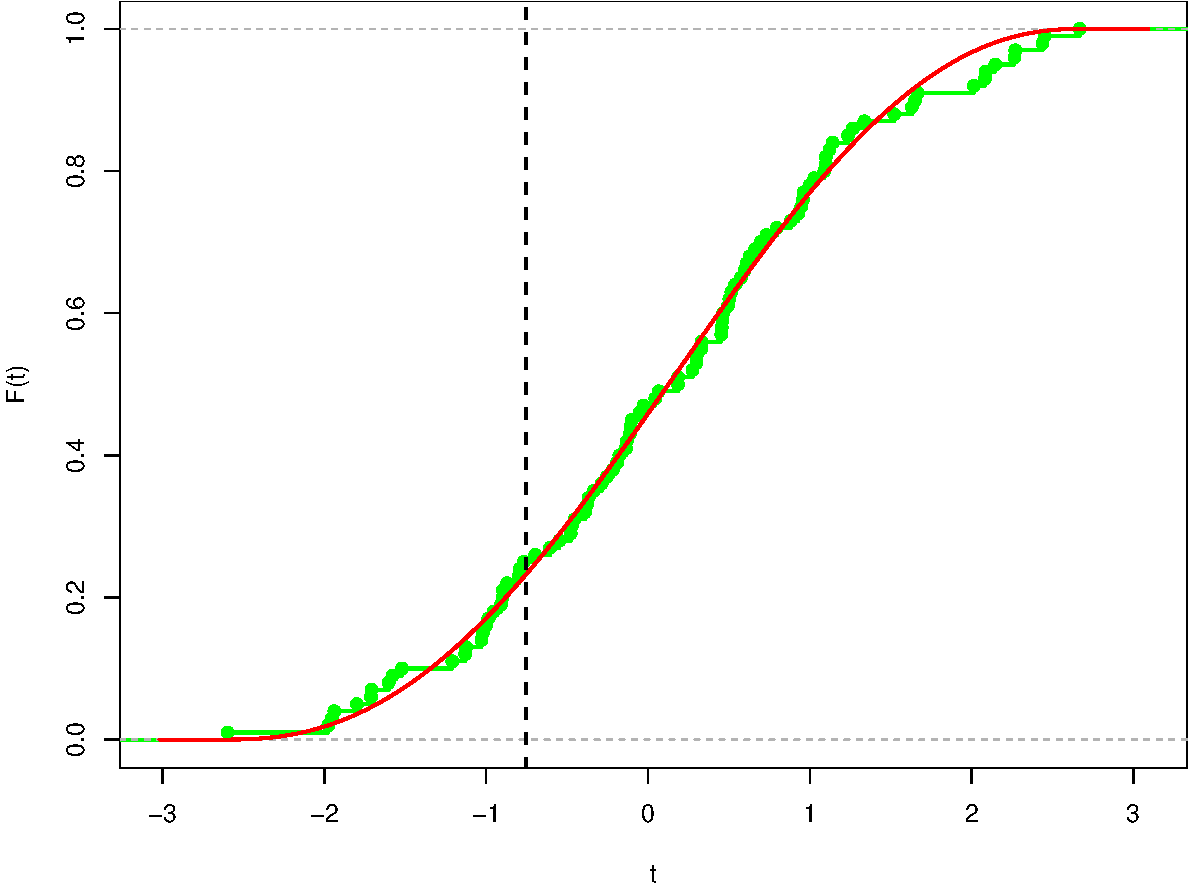
\includegraphics[width=0.6\linewidth]{fig/4-teststat}
	\caption{MC simulation (green) and a Sinusoidal modelling (red) of the classical Student's t-statistic when underlying data distribution came from an unconventional $\Sinu(a_0, 2,3,4)$ distribution.}
	\label{fig:teststat}
\end{figure}



\subsection{Discussion}

Our procedure empirically replaces the classical Student's-t approximation with a data-adaptive Sinusoidal approximation of finite-sample $H_0$ distribution of the t-statistic. Unlike the usual t-test, this method does not rely upon exact Normality of the observations.

The approach may be interpreted as a \textbf{parametric bootstrap} strategy in which both the underlying data distribution as well as the induced statistic distribution are modelled Sinusoidally.

As the sample size increases, one may expect convergence toward the usual Gaussian asymptotics under suitable regularity conditions. However, in small or moderate samples arising from strongly non-Normal populations, the sinusoidal approximation may provide improved p-values and rejection probabilities.